\documentclass[a4paper,12pt]{report}
\usepackage[portuges]{babel}
\usepackage[utf8]{inputenc}
\usepackage{graphicx}
\usepackage{textcomp}
\usepackage[pdftex]{hyperref}
\title{Projeto LightBot - Relatório}
\author{Dinis Peixoto A75353 \and Marcelo Miranda A74817}
\date{\today}

\begin{document} 


\maketitle


\tableofcontents


\chapter{Introdução}
Este trabalho foi nos requerido pelos docentes da unidade curricular \emph{Laboratórios de Informática I} e visa a execução de um jogo já existente (Lightbot) utilizando maioritariamente a linguagem de programação \emph{Haskell}, estudada numa unidade curricular adjacente a esta, \emph{Programação Funcional}. Além desta linguagem, os alunos necessitaram de ficar confortáveis com outras linguagens como \LaTeX, para a execução do relatório, Batch para uma melhor interação com os programas de compilação/interpretação assim como o Sistema de Controle de Versões (SVN), e por fim \textsc{X3DOM} para a animação do jogo. 
Foi também necessário o recurso a uma plataforma, para além da habitual Blackboard, que nos permitiu uma avaliação quantitativa automática, com base em testes predefinidos que tinham como objetivo demonstrar que o nosso programa resultava numa reposta correta (\textsc{MOOSHAK}).

\chapter{LightBot}
O jogo pode ser encontrado à venda na internet (ex: App Store, Google Play) por aproximadamente 2\texteuro. No entanto foi utilizada pelos alunos a versão gratuita de uma hora apenas.*
O jogo consiste num robot, que encontra o problema de ligar todas as lâmpadas presentes num específico mapa, para isso estão disponíveis diversos comandos que podemos utilizar, criando uma sequência que posteriormente o robot realizará. Cada nível chega ao fim quando todas as lâmpadas presentes estão acesas, segue-se outro nível geralmente com um mapa distinto e a dificuldade acrescida.

*\url{http://lightbot.com/hocflash.html}
\begin{figure}[!h]
\centering
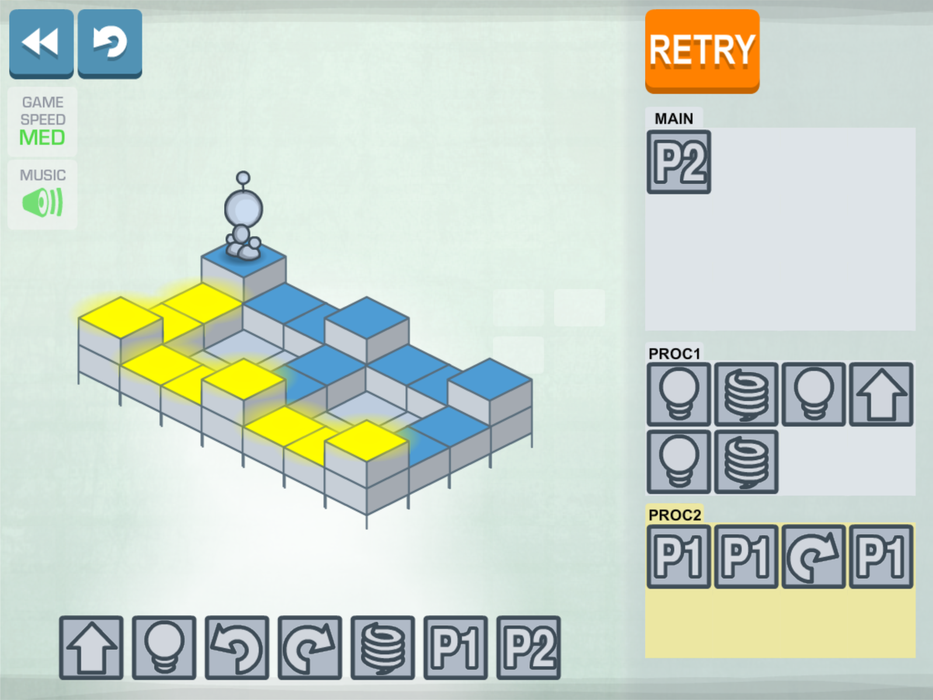
\includegraphics[scale=0.33]{./lightbot.png}
\caption{Imagem do jogo.}
\end{figure}

\chapter{Análise do problema} 
As tarefas solicitadas para este trabalho, tinham objetivos completamente diferentes e, apesar de apresentarem input’s semelhantes, os output’s eram distintos entre si.

\section{Tarefa A}
A tarefa A tinha como objetivo verificar a validade de um determinado input apresentado, tendo em conta que este teria obrigatoriamente de ser composto por uma mapa (que poderia ocupar ou não várias linhas) seguido de uma linha com a posição inicial assim como a orientação do robot e por fim uma linha com os comandos que o robot deveria executar. O output desta tarefa seria \emph{OK} se o input apresentado fosse válido, ou então um número correspondente ao número da linha onde se encontrava o erro, que não permitia a validade do mesmo.
\begin{figure}[!h]
\centering
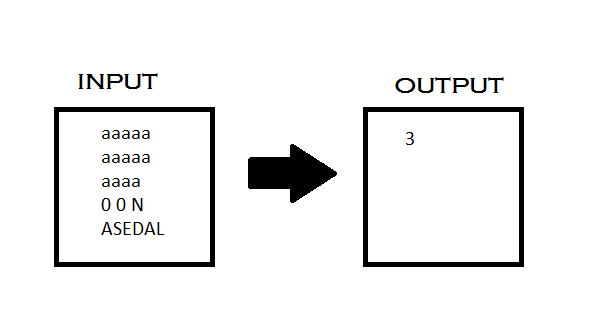
\includegraphics[scale=0.45]{./RELATORIOEX1.png}
\caption{Exemplo de um input inválido e respectivo output.}
\end{figure}

\begin{figure}[!h]
\centering
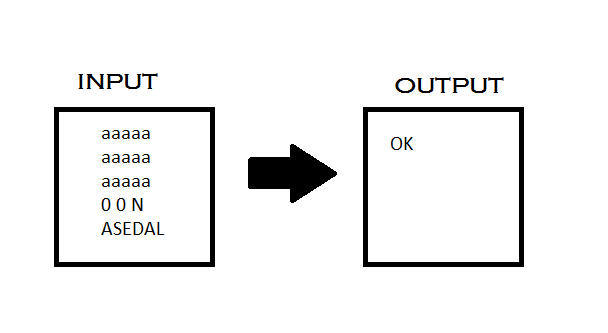
\includegraphics[scale=0.45]{./RELATORIOEX2.png}
\caption{Exemplo de um input válido e respectivo output.}
\end{figure}

\section{Tarefa B}
A tarefa B tem o objetivo de implementar os comandos no jogo, para isso foi-nos proposto o cálculo da próxima posição do robot após um determinado comando. Por sua vez o output desta tarefa, correspondia apenas à posição e respectiva orientação do robot após a execução do primeiro comando, ou caso isto não fosse possível a mensagem \emph{ERRO}. 

\begin{figure}[!h]
\centering
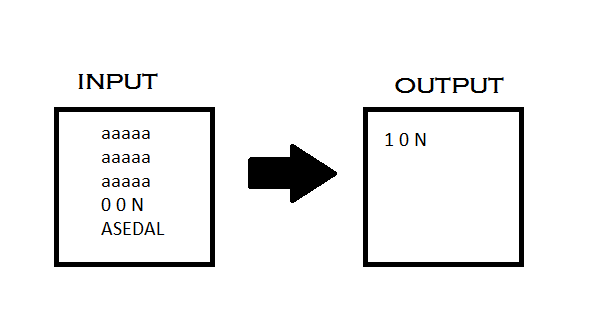
\includegraphics[scale=0.45]{./RELATORIOEX3.png}
\caption{Exemplo de um input válido e respectivo output.}
\end{figure}

\begin{figure}[!h]
\centering
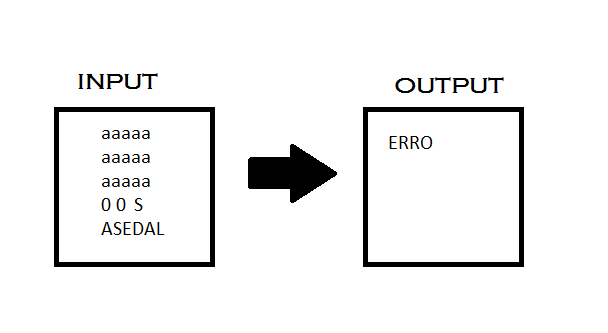
\includegraphics[scale=0.45]{./RELATORIOEX4.png}
\caption{Exemplo de um input inválido e respectivo output.}
\end{figure}



\section{Tarefa C}
A tarefa C é uma tarefa onde a dificuldade cresce exponencialmente e é nada mais que a conclusão da tarefa A e B. Consiste em fazer o robot completar o mapa com que é confrontado, executando os comandos dados. Para isso o robot tem de ligar todas as lâmpadas presentes neste. O input será idêntico ao das tarefas anteriores, já o output será as coordenadas das lâmpadas ligadas seguidas de uma mensagem que pode variar, caso o robot tenha executado um número suficiente de comandos para completar o nível, ligando assim todas as lâmpadas a mensagem imprimida será \emph{FIM \flq número de jogadas válidas\frq}, caso os comandos fornecidos não sejam suficientes para finalizar o nível em que o robot se encontra, deverá ser imprimida a mensagem \emph{INCOMPLETO}.

\begin{figure}[!h]
\centering
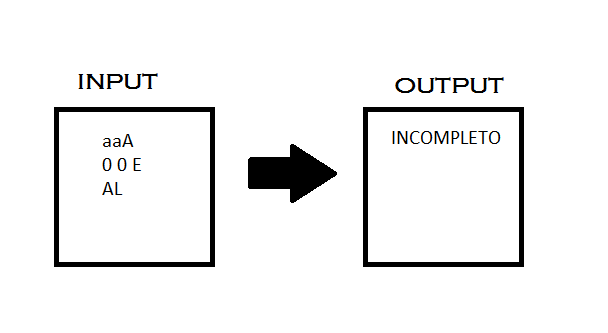
\includegraphics[scale=0.45]{./RELATORIOEX5.png}
\caption{Exemplo de um input inválido e respectivo output.}
\end{figure}

\begin{figure}[!h]
\centering
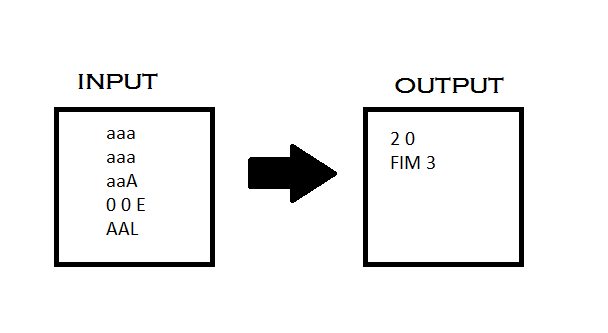
\includegraphics[scale=0.45]{./RELATORIOEX6.png}
\caption{Exemplo de um input válido e respectivo output.}
\end{figure}

\section{Tarefa D}
Completo o jogo em si, segue-se uma nova barreira a ultrapassar. Na tarefa D era pretendido que dado um determinado mapa e uma posição inicial e orientação do robot, o nosso programa conseguisse gerar por si só a linha de comandos que o robot teria de executar para conseguir completar o mapa. 

\begin{figure}[!h]
\centering
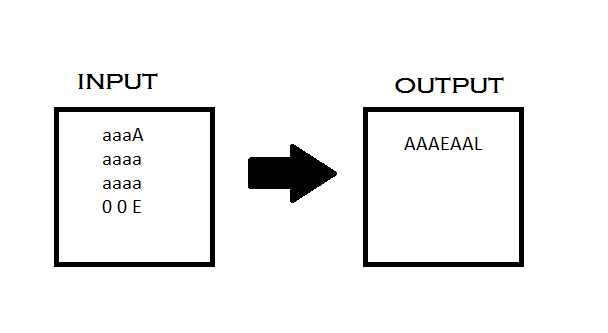
\includegraphics[scale=0.45]{./RELATORIOEX7.png}
\caption{Exemplo de um input e respectivo output.}
\end{figure}

\section{Tarefa E}
Por fim, a tarefa E consiste na criação de um programa em Haskell, tal como nas tarefas antecedentes, que gerasse a animação do jogo. O input desta tarefa é análogo ao das três primeiras tarefas, no entanto o output é completamente distinto das tarefas anteriores, visto ser apresentado como um ficheiro \emph{xhtml} (\textsc{X3DOM}) para ser visualizado como uma página web. 

\begin{figure}[!h]
\centering
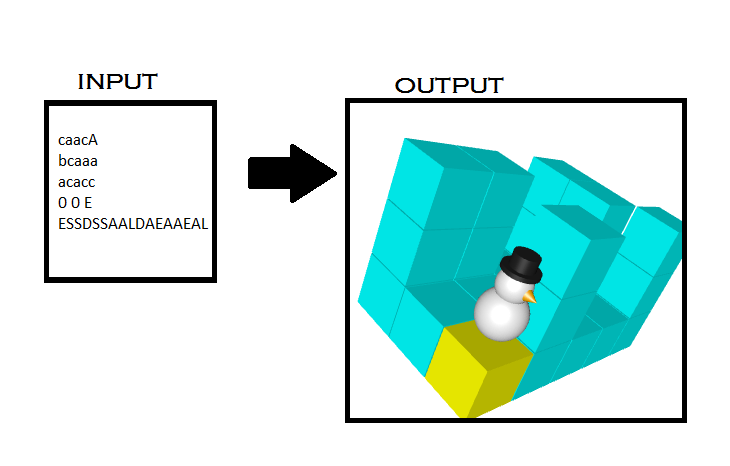
\includegraphics[scale=0.45]{./RELATORIOEX8.png}
\caption{Exemplo de um input e imagem do respectivo output.}
\end{figure}

\chapter{Desenvolvimento do projecto}

\section{Tarefa A}
Para um determinado input ser válido, teria de apresentar as seguintes características: 

\begin{itemize}
\item O mapa corresponderá a uma matriz com um número de linhas independente, mas com um número de colunas idêntico em cada linha. Será constituído exclusivamente por caracteres alfabéticos, que identificarão diferentes níveis (ex: “a” ao nível 0, “b” ao nível 1…), os caracteres devem também representar um outro aspecto, quando forem letra maiúscula estarão a indicar-nos a existência de uma lâmpada. 
\item a linha que se segue ao mapa deverá apresentar as coordenadas x e y da posição Inicial assim como a orientação, utilizando para esta última os pontos cardeais.
\item a linha de comandos deverá ser composta exclusivamente pelas letras iniciais dos comandos mais básicos presentes no jogo: A, E, D, S e L (avançar, esquerda, direita, saltar e lâmpada, respetivamente).
\end{itemize}

\section{Tarefa B}
Na realização desta tarefa, tomamos o tabuleiro como válido, cumprindo assim todos os aspetos da tarefa A.

\begin{itemize}
\item os comandos E e D não alteram a posição do robot, apenas a sua orientação. Também o comando L não provoca qualquer alteração na posição do robot, a função responsável pela execução deste comando, certifica-se apenas de que quando é utilizado o robot se encontra numa posição onde se encontra uma lâmpada.
\item para a realização dos comandos A e S temos de assegurar que a posição resultante após a execução destes comandos será uma posição válida, isto é, uma posição do tabuleiro/mapa e não fora deste. O cálculo da posição resultante é feito consoante a orientação do robot.
\item o comando S requere uma outra condição, a posição seguinte terá de ser inferior à inicial (independentemente do nível) ou, um e um só nível superior à posição anterior.
\item garantir a mensagem \emph{ERRO} quando a posição após o comando não cumpre os requisitos previstos ou quando o comando é utilizado incorretamente, como utilizar “L” numa posição sem lâmpada.
\end{itemize}

\section{Tarefa C}
Nesta tarefa o nosso programa deveria criar uma sequência de comandos, aproveitando assim em grande parte a tarefa B, foi também necessário que recolhesse todas as lâmpadas presentes no tabuleiro/mapa e as inserisse numa lista. As lâmpadas seriam removidas desta lista à medida que fossem acesas, e daríamos o nível por completo quando a lista se encontrava vazia.
Tivemos de considerar algumas situações particulares, como por exemplo:
\begin{itemize}
\item o facto do robot poder desligar uma lâmpada depois desta estar acesa.
\item os comandos que dão erro não devem ter qualquer efeito no robot, e devem portanto ser ignorados. 
\item assegurar a contagem de movimentos válidos.
\end{itemize}

\section{Tarefa D}
Esta tarefa está divida em casos mais simples: em que o robot procura apenas igualar as coordenadas da sua posição às da posição da lâmpada, existindo para isso diversos caminhos e não encontrando obstáculos muito preocupantes à sua deslocação, isto é, posições com dois níveis superiores. E casos mais complicados, onde tivemos de encontrar uma resolução para situações em que existem: 
\begin{itemize}
\item elevadas discrepâncias entre níveis;
\item lâmpadas com um único acesso;
\item posições que levariam o robot a não conseguir executar mais comandos.
\end{itemize}

\section{Tarefa E}
O programa relativo a esta tarefa tinha como objetivo gerar a animação do jogo em \textsc{X3DOM}. Esta tarefa foi realizada por etapas:
\begin{description}
\item[1]Gerar o mapa.
\item[2]Gerar o boneco.
\item[3]Gerar o mapa, bonecos e sucessivos movimentos realizados por este (opcional).

\end{description}
Como não tínhamos qualquer conhecimento em \textsc{X3DOM}/\textsc{HTML}, fomos utilizando o código fornecido pelos docentes da unidade curricular, conforme os nossos objetivos. 

\chapter{Conclusão}
Ambos os membros do grupo consideram este projeto como algo essencial ao curso em que se encontram. Reconhecemos que foi uma experiência enriquecedora, porque além de ser o nosso primeiro contacto com a programação, obrigou-nos a ter uma atitude mais autónoma, que nos levou à procura de novas funções para por vezes nos facilitar o trabalho, mas principalmente na última tarefa em que nos foram requisitados conhecimentos básicos sobre \textsc{X3DOM} que nunca tínhamos abordado numa unidade curricular. 
A última tarefa permitiu-nos também visualizar graficamente grande parte do trabalho que até então não passava de meras linhas de código, foi como uma recompensa ao fim de inúmeras horas dedicadas ao trabalho.


\end{document}